
%%%%%%%%%%%%%%%%%%%%%%%%%%%%%%%%%%%%%%%%%%%%%%%%%%%%%%%%%%%%%%%%%%%%%%%%%%%%%
%%%%% Half-edge Data Structure %%%%%%%%%%%%%%%%%%%%%%%%%%%%%%%%%%%%%%%%%%%%%%
%%%%%%%%%%%%%%%%%%%%%%%%%%%%%%%%%%%%%%%%%%%%%%%%%%%%%%%%%%%%%%%%%%%%%%%%%%%%%
\fbckg{backgrounds/blank2}
\setbeamercolor{frametitle}{fg=gray}
\begin{frame}
\pointedsl{
	Half-Edges
}
\end{frame}

%
% Content:
% 1. What is a half-edge?
% 2. How are elements connected?
% 3. How do I work with half-edges?
% 4. How do I work with vertices? faces? edges?

%%%%%%%%%%%%%%%%%%%%%%%%%%%%%%%%%%%%%%%%%%%%%%%%%%%%%%%%%%%%%%%%%%%%%%%%%%%%%
\begin{frame}
\frametitle{Half-edges}
\begin{center}
	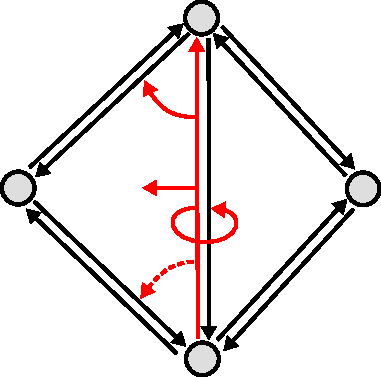
\includegraphics[width=0.5\textwidth]{figures/halfedge-connectivity}
\end{center}
\misc{
	Meshes are made of \emph{vertices}, \emph{edges} and \emph{faces}.
	
	Here, each edge is made of two \textbf{half-edges} (directed edges).
}
\end{frame}

%%%%%%%%%%%%%%%%%%%%%%%%%%%%%%%%%%%%%%%%%%%%%%%%%%%%%%%%%%%%%%%%%%%%%%%%%%%%%
\begin{frame}
\frametitle{Connectivity}
\begin{columns}[c]
  \begin{column}{0.4\textwidth}
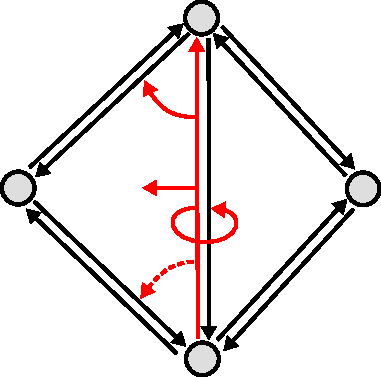
\includegraphics[width=\textwidth]{figures/halfedge-connectivity}
  \end{column}
  \begin{column}{0.6\textwidth}
\begin{itemize}
	\color{black}
	\item[\color{black}\textbullet] Each \textbf{vertex} is linked to an outgoing half-edge
	\item[\color{black}\textbullet] Each \textbf{face} is linked to an incident half-edge
	\item[\color{black}\textbullet] Each \textbf{half-edge} has \begin{itemize}
		\color{black}
		\item[\color{black}\textbullet] A next and previous half-edge
		\item[\color{black}\textbullet] A target vertex it points to
		\item[\color{black}\textbullet] An incident face
		\item[\color{black}\textbullet] An opposite half-edge\\(on the same edge)
	\end{itemize}
	\item[\color{black}\textbullet] Each \textbf{edge} has two corresponding half-edges
\end{itemize}
  \end{column}
\end{columns}
\end{frame}

%%%%%%%%%%%%%%%%%%%%%%%%%%%%%%%%%%%%%%%%%%%%%%%%%%%%%%%%%%%%%%%%%%%%%%%%%%%%%
\begin{frame}[fragile]
\frametitle{Half-edges code}
\begin{columns}[c]
  \begin{column}{0.4\textwidth}
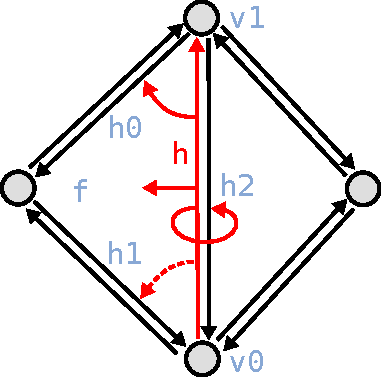
\includegraphics[width=\textwidth]{figures/halfedge-queries}
  \end{column}
  \begin{column}{0.6\textwidth}
  \lstset{ 
  	numbers=none, 
  	xleftmargin=0cm, 
  	xrightmargin=0cm
  }
\begin{lstlisting}
using Surface_mesh::Halfedge;
using Surface_mesh::Face;
using Surface_mesh::Vertex;

// the starting half-edge
Halfedge h;
// the connected elements
Halfedge h0, h1, h2;
Face f;
Vertex v0, v1;
\end{lstlisting}
  \end{column}
\end{columns}
\end{frame}

\begin{frame}[fragile]
\frametitle{Half-edges code}
\lstset{ numbers=none }
\begin{lstlisting}
// next half-edge
h0 = mesh.next_halfedge(h);
// previous half-edge
h1 = mesh.prev_halfedge(h);
// opposite half-edge
h2 = mesh.opposite_halfedge(h);
// incident face
f = mesh.face(h);
// vertex at source
v0 = mesh.from_vertex(h);
// vertex pointed by h
v1 = mesh.to_vertex(h);
\end{lstlisting}
\end{frame}

%%%%%%%%%%%%%%%%%%%%%%%%%%%%%%%%%%%%%%%%%%%%%%%%%%%%%%%%%%%%%%%%%%%%%%%%%%%%%
\begin{frame}[fragile]
\frametitle{Vertices, edges and faces}
\lstset{ numbers=none }
\begin{lstlisting}
// half-edge h of vertex v
h = mesh.halfedge(v);

// edge e of half-edge h
e = mesh.edge(h);
// half-edges h0,h1 from edge e
h0 = mesh.halfedge(e, 0);
h1 = mesh.halfedge(e, 1);

// half-edge h of face f
h = mesh.halfedge(f);

// checking if at the boundary
// same for h, e, f, v
bool b = mesh.is_boundary(h);
\end{lstlisting}
\end{frame}